\documentclass{article}
\usepackage{amsmath}
\usepackage{amsfonts}
\usepackage{amsthm}
\usepackage{parskip}
\usepackage{chngcntr}
\usepackage{textgreek}
\usepackage{graphicx}
\graphicspath{ {./images/}  }
\counterwithin*{section}{part}
\begin{document}
\title{Lectures Notes for Calculus}
\author{Emulie Chhor}
\maketitle

\section*{Introduction}

\section{Why Study Calculus?}

\section{Overview of Calculus}

Le Calcul se découle en 4 cours:

    \begin{enumerate}
	\item Calcul Différentiel
	\item Calcul Intégral
	\item Calcul à Plusieurs Variables
	\item Vector Calculus
    \end{enumerate}

Le premier cours de calcul porte sur les limites, la continuité et la
différentiabilité. Puisqu'il s'agit d'un premier cours de calcul, une grande
partie est axée sur le calcul des limites et la dérivations et ses applications.
C'est dans le cours d'analyse qu'on prend une approche plus rigoureusement les
notions de limites, continuité et différentiabilité.

Le deuxième cours de calcul porte sur les techniques d'intégrations et les suites
et séries.

Le troisième cours de calcul porte encore sur les limites, la convergence,
la continuité et la différentiabilité, mais on ajoute une 3e dimension. On verra
comment utiliser les coordonnées polaires et cartésiennes pour changer les bornes
d'intégrations et visualiser les intégrales à dessiner.

Finalement, le quatrième cours de calcul porte sur le Vector Calculus.

\pagebreak

\newtheorem{definition}{Definition}[subsection]
\newtheorem{theorem}{Theorem}[subsection]
\newtheorem{corollary}{Corollary}[subsection]
\newtheorem{lemma}[theorem]{Lemma}
\newtheorem{proposition}{Proposition}[section]
\newtheorem{axiom}{Axiome}
\newtheorem{property}{Propriété}[subsection]
\newtheorem*{remark}{Remarque}
\newtheorem*{problem}{Problème}
\newtheorem*{intuition}{Intuition}

\part{Pre-Calculus}
\section{Overview}
\pagebreak

\part{Calcul Différentiel}

\section{Overview}

Le calcul différentiel se découle en plusieurs chapitres:

\begin{enumerate}
    \item Fonctions
    \item Limites et Continuité
    \item Dérivées
    \item Applications des dérivées
\end{enumerate}

\section{Fonctions}
\subsection{Détermination du domaine, des zéros et du graphe d’une fonction}
\subsection{Caractéristiques des fonction algébriques et transcendantes usuelles}
\section{Limites et continuité}
\subsection{Notion informelle de limite}
\subsection{Calcul des limites}
\subsection{Formes indéterminées}
\subsection{Continuité d’une fonction}

\section{Dérivées}
\subsection{Définition en terme de limite}
\subsection{Calcul de la dérivée à l’aide de limites}
\subsection{Propriétés des dérivées}
\subsection{Formules de dérivation}
\subsection{Calcul de dérivées à l’aide des formules}
\subsection{Dérivée des fonctions transcendantes}
\subsubsection{Fonctions Trigonométriques}
\subsubsection{Fonctions Trigonométriques Inverses}
\subsubsection{Fonctions Exponentielles}
\subsubsection{Fonctions Logarithmique}
\subsection{Dérivation implicite}

\section{Applications des dérivées}
\subsection{Croissance et décroissance}
\subsection{Maximums et minimums}
\subsection{Concavité et points d’inflexion}
\subsection{Tableau de variation et graphes de fonctions}
\subsection{Asymptotes verticales et horizontales}
\subsection{Optimisation}

\pagebreak

\part{Calcul Intégral}

\section{Overview}

Le calcul intégral se découle en plusieurs chapitres:
\begin{enumerate}
    \item Introduction aux Intégrales
    \item Fonctions exponentielles, logarithmiques, trigos et inverses trigos
    \item Techniques d'intégration
    \item Applications d'Intégration
    \item Équations différentielles
    \item Suites et Séries
\end{enumerate}

\section{Limites, continuité et dérivées}
\subsection{Dérivation logarithmique}
\subsection{Règle de l’Hospital}
\subsection{Différentielles}
\section{Intégrale indéfinie}
\subsection{Équations différentielles à variables séparables}
\subsection{Formules d’intégration}
\subsection{Changement de variable}
\section{Intégrale définie}
\subsection{Notation sigma}
\subsection{Sommes de Riemann}
\subsection{Théorème fondamental du calcul}
\subsection{Changement de variable}
\section{Techniques d’intégration}
\subsection{Intégration par parties}

La technique d'intégration par parties est une technique d'intégration utile
lorsqu'on a un produit de fonction avec u facile à dériver et dv facile à
intégrer.

\begin{theorem}[Intégration par parties]
    $$ \int u dv = uv - \int v du $$
\end{theorem}

\begin{remark}[Intégrale par parties cirulaire]
    Parfois, on obtient la même équation de part et d'autres de l'équation,
    alors on peut isoler et résoudre algébriquement,
\end{remark}

\subsection{Intégrale trigonométrique}

Lorsqu'on doit résoudre des intégrales trigos, qui sont des intégrales
écrites uniquement avec des fonctions trigos (ou inverse trigos?), on
utilise les identité trigos pour substituer pour exprimer la fonction en
une seule fonction trigo (et utiliser substitution u)

Habituellement, on regarde la la parité de l'exposant pour déterminer quelle
stratégie utiliser.

\begin{enumerate}
    \item si m pair et n impair: on utilise
	$ sin^2(\theta) + cos^2(\theta) = 1$
    \item si m et n sont pair: on remplace $cos^2x$ et $sin^2(x)$
    \item si m en n sont impair: $ sin(x) cos(x) = \frac{1}{2} sin(2x)$
    \item si m et n ont le même exposant:
    \item si a et b prennent des valeurs différentes
\end{enumerate}

\begin{theorem}[Identités trigos]
    \begin{enumerate}
	\item $ sin^2(\theta) + cos^2(\theta) = 1$
	\item $ sec^2(\theta) = 1 + tan^2(\theta) $
	\item $ cos^2(x) = \frac{1}{2} (1+cos(2x))$
	\item $ sin^2(x) = \frac{1}{2} (1-cos(2x))$
	\item $ sin(x) cos(x) = \frac{1}{2} sin(2x)$
	\item $ sin(a) cos(b) = \frac{1}{2} [sin(a-b) + sin(a+b)]$
	\item $ sin(a) sin(b) = \frac{1}{2} [cos(a-b) - cos(a+b)]$
	\item $ cos(a) cos(b) = \frac{1}{2} [cos(a-b) + cos(a+b)]$
    \end{enumerate}
    \begin{enumerate}
	\item $ cos(-A) = cos(A)$
	\item $ sin(-A)= - sin(A)$
	\item $ sin(A+B) = sin(A) \cdot cos(B) + cos(A) \cdot sin(B)$
	\item $ sin(A-B) = sin(A) \cdot cos(B) - cos(A) \cdot sin(B)$
	\item $ cos(A+B) = cos(A) \cdot cos(B) - sin(A) \cdot sin(B)$
	\item $ cos(A-B) = cos(A) \cdot cos(B) + sin(A) \cdot sin(B)$
    \end{enumerate}
\end{theorem}

\begin{remark}
    On obtient l'indentité $ sec^2(\theta) = 1 + tan^2(\theta) $ en divisant
    $ sin^2(\theta) + cos^2(\theta) = 1$ par $ cos^2x$ de chaque côté.
\end{remark}

\subsection{Substitution trigonométrique}

Parfois, même avec des u-substitution, il n'est pas possible de résoudre
l'intégrale, car on est encore pris avec la racine. Ainsi, on veut utiliser
le lien entre les propriétés trigos (algébriques) et le théorème de
pythagore pour pouvoir se débarasser de la racine.

\subsubsection{Intuition derrière la substitution trigo}%
\label{ssub:Intuition derrière la substitution trigo}

Le premier concept à se souvenir est qu'on veut partir des identités trigos
pour construire notre triangle et poser u. En appliquant la racine des 2
côtés, on obtient:
\begin{enumerate}
    \item $ 1-sin^2(\theta) = cos^2(\theta) \Longrightarrow
	\sqrt{1-sin^2(\theta)} = cos(\theta)$
    \item $ sec^2(\theta) = 1 + tan^2(\theta) \Longrightarrow
	\sqrt{1+tan^2(\theta)} = sec(\theta)$
    \item $ sec^2(\theta) - 1 = tan^2(\theta) \Longrightarrow
	\sqrt{tan(\theta)}$
\end{enumerate}

Ainsi, on veut poser u pour satisfaire

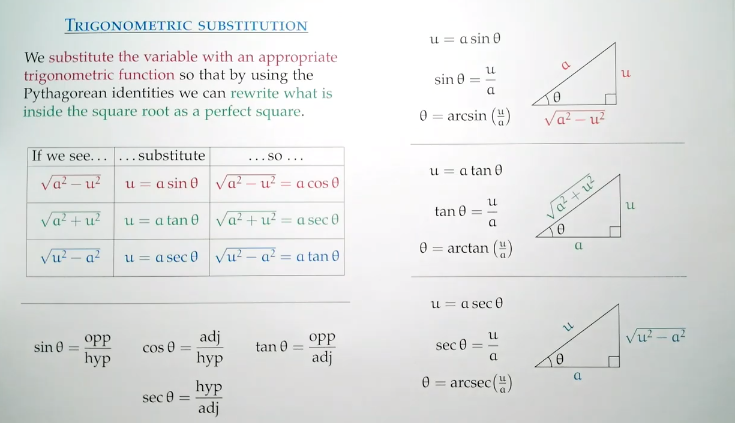
\includegraphics{trigonometric_substitution_butler}

\subsubsection{Méthodologie pour la substitution trigo}%
\label{ssub:}

\begin{enumerate}
    \item Essayer de résoudre avec substitution u ou autre
    \item Déterminer quelle forme trigo on a pour poser $\theta$
	p/r à x
    \item Calculer la dérivée de $\theta$
    \item Substituer par theta et changer les bornes d'intégration si on
	a une intégrale définie.
    \item Résoudre
    \item Réécrire l'intégrale p/r à la variable d'origine x à l'aide du
	triangle ou algébriquement.
\end{enumerate}

\begin{remark}[Comment retrouver la variable de début]

\end{remark}

\subsection{Décomposition en fractions partielles}

\begin{enumerate}
    \item Équation linéaire
    \item Équation quadratique
\end{enumerate}

\section{Applications de l’intégrale définie}
\subsection{Aire entre deux courbes}
\subsection{Volume de solides de section connue}
\subsection{Surfaces et volumes de révolution}
\subsection{Longueur d’une courbe}
\section{Suites et séries}
\subsection{Suites — définition et notion de convergence}
\subsection{Séries — définition}
\subsection{Séries Notables}
\subsection{Critères de convergence}
\subsubsection{Séries à termes positifs}
\subsubsection{Séries alternées}
\subsection{Séries de puissance}
\subsubsection{Séries de Taylor et de MacLaurin}

\pagebreak

\part{Calcul à plusieurs variables}
\section{Overview}

Le calcul à plusieurs varaibles se découle en plusieurs chapitres:

\begin{enumerate}
    \item Vecteurs et Matrices
    \item Équations des droites et des plans
    \item Fonctions de plusieurs variables
    \item Equations Paramétriques et Coordonnées Polaires
    \item Dérivées Partielles
    \item Optimisation
    \item Intégrales Multiples
\end{enumerate}
\pagebreak

\section{Vecteurs et Matrices}
\section{Équations des droites et des plans}
\section{Fonctions de plusieurs variables}
\section{Equations Paramétriques et Coordonnées Polaires}

\subsection{Coordonnées Polaires}%
\label{ssub:Coordonnées Polaires}

\subsubsection{Overview}%
\label{ssub:Overview}

Les coordonnées polaires est une transformation cartésienne qui rend
les coordonnées de la base en cercle. Dans un sytème de coordonnées
cartésiennes, on décrit les vecteurs p/r à distance-distance, alors que
dans un système de coordonnées polaires, on décrit les vecteurs en
terme de distance-direction. Les coordonnées polaires sont pratiques, car
on peut décrire plusieurs vecteurs par leur directions.

\subsubsection{D'où vient les coordonnées polaires}%
\label{ssub:D'où vient les coordonnées polaires}

À l'aide d'un triangle rectangle dont les côtés sont x et y, on obtient que
$ x^2 + y^2 = r^2$, où r est l'hypothénuse. On obtient donc les relations
suivantes:
\begin{enumerate}
    \item $x=rcos(\theta)$
    \item $x=rsin(\theta)$
    \item $tan(\theta) = \frac{y}{x} $
\end{enumerate}

\begin{problem}
    \begin{enumerate}
        \item Sketch the curve: TODO
    \end{enumerate}
\end{problem}


\section{Dérivées Partielles}
\section{Optimisation}
\section{Intégrales Multiples}


\part{Vector Calculus}
\section{Overview}
\pagebreak

\part{Ressources} % (fold)%
\label{prt:Ressources}

\section{Books}%
\label{sec:Books}

\section{Lectures}%
\label{sec:Lectures}

\begin{enumerate}
    \item Professor Butler Calculus I,II,III: well structured courses with a
	website+exercices, and each theoritical class is accompanied by a
	practice class (recommended)
	\url{https://www.calc2.org/videos/fall-20-online-w-butler}
\end{enumerate}

\section{Exercices}%
\label{sec:Exercices}

\begin{enumerate}
    \item Paul's Lectures Notes
\end{enumerate}

% part Ressources (end)

\end{document}
\end{article}
